\documentclass[british,titlepage]{ntnuthesis}

\title{Long-term vessel trajectory inference using Gaussian Processes }
\shorttitle{Gaussian Process Trajectory Inference}
\author{%
Håvard Skåra Mellbye
\vspace{1cm}\\
Supervisor: Edmund Førland Brekke \\ 
Co-supervisor: Trym Tengesdal
}
\shortauthor{Mellbye}
\date{}


\addbibresource{thesis.bib}

\usepackage{tikz}
\usetikzlibrary{bayesnet}
\usepackage{ifthen}


% From https://www.overleaf.com/learn/latex/Glossaries

\makeglossaries % Prepare for adding glossary entries



% --------------------
% ----- Acronyms -----
% --------------------

\newacronym{gp}{GP}{Gaussian Process}
\newacronym{mcmc}{MCMC}{Markov Chain Monte Carlo}
\newacronym{pgm}{PGM}{Probabilistic Graphical Model}
\newacronym{bp}{BP}{Belief Propagation}
\newacronym{dgm}{DGM}{Directed Graphical Model}
\newacronym{bn}{BN}{Bayesian Network}
\newacronym{mrf}{MRF}{Markov Random Field}
\newacronym{kl}{KL}{Kullback-Liebler divergence}
\newacronym{pdf}{PDF}{Probability Density Function}
\newacronym{pmf}{PMF}{Probability Mass Function}
\newacronym{vi}{VI}{Variational Inference}
\newacronym{elbo}{ELBO}{Evidence Lower Bound}
\newacronym{hmc}{HMC}{Hamiltonian Monte Carlo}
\newacronym{nuts}{NUTS}{No-U-Turn sampler}
\newacronym{colav}{COLAV}{Collision Avoidance}
\newacronym{ml}{ML}{Machine Learning}
\newacronym{sog}{SOG}{Speed Over Ground}
\newacronym{cog}{COG}{Course Over Ground}
\newacronym{rbf}{RBF}{Radial Basis Function}

\newglossaryentry{moralization}
{
    name=moralization,
    description={The process of converting Directed Graphical Models into Markov Random Fields}
}

\newglossaryentry{support}{
    name=support,
    description={The set of possible outcomes/values with a non-zero probability, i.e. all events that can happen. A Gaussian distribution for example have support for $x \in \mathcal{R}$ since it has a non-zero probability, $p(x) > 0$, for all real numbers $x \in \mathcal{R}$.}
}

\newglossaryentry{colregs}{
    name=COLREGS,
    description={International Regulations for Preventing Collisions at Sea, a set of rules for ships navigating at sea.}
} % add glossary and acronym lists before document

\begin{document}

\chapter*{Abstract}

Autonomous ships depend on situational awareness in order to avoid collisions in a safe and robust manner. By knowing the intention of surrounding vessels, safety margins can be improved by avoiding situations with increased risk. In this thesis, methods for Bayesian Inference will be explored, with the goal of developing a flexible framework for intention modelling. Exact and approximate inference methods are explored. Approximate methods are found to be more flexible, allowing easier incorporation of existing knowledge from domain experts or conventions such as \Gls{colregs}. Methods such as \acrfull{mcmc} and \acrfull{vi} are therefore explored further and compared on an illustrative intention model. The results then find \acrshort{mcmc} to be accurate at the cost of computational complexity. \acrshort{vi} on the other hand, is found to be a lot faster, though much less precise on the illustrative model. 

\tableofcontents
\listoffigures
\listoftables
%\lstlistoflistings


\printglossary[type=\acronymtype] % Print acronyms
\printglossary                    % Print glossary

\chapter{Introduction}

Humans, while resourceful, are prone to loss of focus, tiredness and have limited attention span. Human errors are estimated to contribute to more than $75\%$ of maritime accidents \cite{Tengesdal2020RiskbasedAM}. On the contrary, computers always remain "focused" and never gets tired. Using autonomus ships in order to reduce the potential for human errors can greatly reduce the number of maritime accidents.
While completely avoiding humans at sea would increase safety, it simply is unrealistic. Autonomous ships will need cooperate with humans on nearby vessels to avoid dangerous situations. Such up-to-date situational awareness is critical to develop decision-making systems in dynamic environments \cite{endsley}. Robust \acrfull{colav} are necessary to  maneuver in areas with potential obstacles in order to avoid collisions. However, the optimal decision is usually highly situation-dependent and requires ability to understand and predict the traffic patterns of nearby vessels, either controlled by humans or autonomous. The optimal decision are further influenced by conventions such as \Gls{colregs}, especially for larger vessels. Still, some scenarios may even require rules and conventions to be broken due to unforeseen circumstances.
However, teaching machines situational awareness is not an easy task. Human's remarkable ability to recognize situations from observations is very hard to replicate in an autonomous systems.

\section{Existing research}
 Existing research on intention modelling for autonomous ships is limited. \cite{Tengesdal2020RiskbasedAM} propose a Probabilistic Scenario-Based Model Predictive Control scheme which is able to utilize probabilistic information about obstacle intentions. It demonstrates how it is possible to make safer decisions when utilizing the additional intent information. The paper propose a general framework for intention inference using \acrfull{bn}, allowing several factors to influence an obstacle's intention. However, the paper only propose an illustrative model where the parameters of the model are assumed known and do not further discuss how these models can be found or used in practice.  

Some related research has been made in the area of autonomous cars. \cite{song} explore how Hidden Markov Models (HMM) can be used to infer the intention of cars in an intersection and then utilize this information in a partially observable Markov decision process (POMDP). 


\section{Bayesian Networks}
Bayesian Networks, often called Belief Networks, are Probabilistic Graphical Models represented as directed acyclic graphs \cite{murphy}. There is strictly speaking nothing Bayesian about Bayesian Networks (they may just as well be used with Frequentist statistics), as it is simply a way to describe probability distributions. Bayesian Networks are also often used to represent causal relations, though the interactions are in no way required to be causal. However, the causal interpretation of Bayesian Networks allow humans to intuitively understand relations between variables. Bayesian Networks are for this reason heavily used in Causal Inference, which attempts to model and infer true causal relationships between variables \cite{causal}. Bayesian Networks intuitive structure further allows human domain experts to reason about and participate in the development of statistical models, without requiring deep statistical knowledge. 
This makes Bayesian Networks a good choice for intention models, as the model need to incorporate prior knowledge such as intuitive reasoning, human experts and predefined rules (such as \Gls{colregs}), as well as be able to learn from new and historical observations. 

\section{Goal}
This thesis will investigate how inference can be performed from available data in a Bayesian Network. At this point the goal is not to find a realistic intention model, but rather try to develop a flexible framework for inference in a known model. Methods which makes few assumptions about the model and makes it easy to incorporate existing knowledge will be the main focus of this thesis. This choice comes from a belief that a good intention model will need to strongly rely on prior knowledge from human experts and from predefined rules. Restricting the model by assumptions made by the inference methods, may end up restricting the ability to accurately encode such information into the model. Approximate Methods such as \acrfull{mcmc} and \acrfull{vi} will therefore be explored in greater detail, while exact methods are only presented as possible solutions for special cases where the assumptions are reasonable. The methods can in some cases be combined, by utilizing exact inference wherever the assumptions are reasonable, and fall back to approximate methods on the parts where exact methods falls short \cite{winnbishop}.
This thesis is structured into multiple chapters. Some necessary theoretical background, mainly an introduction to Bayesian Statistics and \acrfull{pgm}'s, are presented in \cref{chap:theory}. The theory for \acrshort{mcmc} based methods are then found in \cref{chap:mcmc}, while exact and approximate analytical methods are found in \cref{chap:analytical}. In order to not only present the theoretical concepts, implementations of \acrshort{mcmc} and \acrshort{vi} are compared on a fictitious model in \cref{chap:impl}. Finally, the theory and results for the different methods are then compared and discussed in \cref{chap:discussion}.
\chapter{Neccessary Theoretical Background}

\section{Useful Results From Probability Theory}

The reader is assumed to have basic understanding of probability theory. Some of the most relevant results are summarized here.
 
 \subsection{Notation}
 
 The notation $p(X)$ is used to denote the probability distribution of the random variable $X$.
 
 For \textbf{discrete} random variables the notation is straight forward. 
 \begin{align*}
 p(X) &= p(X=x)\\  &= p_X(X=x)\\ &= \Pr\{X = x\}
 \end{align*}
 
 For \textbf{continuous} random variables the probability of a single outcome is always zero, i.e. $p(X = x) \equiv 0$, as there are infinitely many possible outcomes. The notation $p(X)$ then denotes the probability density function (PDF) of $X$. 
 
 The notation $\Pr\{\cdot\}$, such as $\Pr\{X=x\}$ and $\Pr\{X \leq x\}$, is used to denote probability of a specific event occurring. The output of this operator is always a probability, i.e. $\Pr\{\cdot\} \in (0, 1)$. 
 
 
 
\subsection{Joint Probabilities}
The \textit{joint probability} $p(X, Y)$ is the probability that both $X$ and $Y$ occurs \cite[p.~29]{murphy}.

\begin{equation}
    p(X, Y) = p(X \cap Y) = p(X | Y)p(Y)
\end{equation}

\subsection{Conditional Probabilities}
The \textit{conditional probability} $p(X | Y)$ is the probability of $X$ occurring, given the known occurrence of another event $Y$. This can be interpreted as knowing the value of $Y$ includes some information about $X$. Mathematically it can be expressed as \cite[p.~29]{murphy}
\begin{equation}\label{eq:conditional_probability}
    p(X | Y) = \frac{p(X, Y)}{p(Y)}
\end{equation}

\subsection{Bayes Rule}

A useful extension to equation \eqref{eq:conditional_probability} is to recognize that the joint distribution $p(X, Y)$ can be rewritten as a product of a conditional probability $p(Y | X)$ and $p(X)$. Inserting into equation \eqref{eq:conditional_probability} yields \textit{Bayes Rule}
\begin{equation}\label{eq:bayes_law}
    p(X | Y) = \frac{p(X, Y)}{p(Y)} = \frac{p(Y | X)p(X)}{p(Y)}.
\end{equation}

As $Y$ is known, the denominator $p(Y)$ is simply a normalizing constant. It is sometimes useful to rewrite equation \eqref{eq:bayes_law} as
\begin{equation}\label{eq:bayes_law_proportional}
    p(X | Y) = \frac{p(Y | X) p(X)}{p(Y)} \propto p(Y | X)p(X)
\end{equation} 
if $p(Y)$ is hard to calculate and the normalized value of $p(X | Y)$ is not needed.

\subsection{Marginal Probability \& The Law of Total Probability}\label{sec:marginal_prob}
The \textit{marginal probability} of an event $X$ is the probability of $X$ occurring irrespective of any other variables.
For notational simplicity the integral operator is used for marginalization of both continuous and discrete random variables, even though the integral is replaced by a sum for discrete random variables. For an event $X$ and any other variables $\bf Y$, the marginal probability of $X$ can be written as
\begin{equation}
    p(X) = \int_{\boldsymbol{Y}} p(X, \boldsymbol{Y}) d\boldsymbol{Y} = \int_{\boldsymbol{Y}} p(X | \boldsymbol{Y}) p(\boldsymbol{Y}) d\boldsymbol{Y}
\end{equation}
The last equality is by the \textit{Law of total probability}, which relates marginal probabilities to conditional probabilities.

\subsection{Independence \& Conditional Independence}
If the joint probability of two variables $X$ and $Y$ can be expressed as a product of two marginals, then they are \textit{marginally independent}.
\begin{equation}
    X \perp Y \iff p(X, Y) = p(X | Y)p(Y) = p(Y | X)p(X) = p(X)p(Y)
\end{equation}

Marginal independence is rare, as most variables usually influence each other in some way. However, the variables often affect one another indirectly through other variables. The variables $X$ and $Y$ are said to be \textit{conditionally independent} given $Z$, if the conditional joint can be written as a product of conditional marginals \cite[p.~31]{murphy}:
\begin{equation}\label{eq:conditional_independence}
    X \perp Y | Z \iff p(X, Y | Z) = p(X | Z)p(Y | Z)
\end{equation}

\subsection{Interpretations of Probability}
The results mentioned so far stem from abstract mathematical axioms, and do not tell how to interpret the resulting probabilities. Different interpretations are commonly accepted. The perhaps two biggest interpretations are the Frequentist and Bayesian interpretations. 

\begin{description}
    \item[The Frequentist Interpretation:] The Frequentists define an event's probability as the limit of its relative frequency over many trials. In other words, the probabilities are assigned a physical interpretation and remains rather objective. There do however arise issues and paradoxes when assigning probabilities to events which are not recurrent, i.e. they only happen a few times. The Frequentist interpretation assumes that the collected data is random and that the model (and its corresponding parameters) are fixed. The main goal of the Frequentists are therefore to create consistent methods for dealing with uncertain data.
    \item[The Bayesian Interpretation:] The Bayesians interpret probability as a state of knowledge \cite{Jaynes86bayesianmethods:}. In Bayesian analysis the data is fixed, whereas the model is unknown. Data is used to update prior knowledge about the model, and the probabilities are used to quantify how strongly one believe in each outcome. This interpretation is highly philosophical, but beautifully captures humans' intuitive reasoning. The Bayesian interpretation does however involve a level of subjectivity when choosing priors, making it difficult to form objective opinions from data. For those interested, see \Cite{Jaynes86bayesianmethods:} for a fascinating read on the history of Bayesian probability.
\end{description}

While the differences between the Frequentist and Bayesian interpretations are mostly philosophical, there are a few practical differences. For a Frequentist it does not make sense to talk about any probabilities before an experiment has been performed. The prior $p(X)$ and posterior $p(X | Y)$ is therefore nonsensical and cannot be computed using a Frequentist interpretation.



\section{Identifiability}



\section{Bayesian Statistics}

Using \cref{eq:bayes_law} one can write 
\begin{equation}\label{eq:bayes_learning}
    p(\boldsymbol{\theta}| \mathcal{D}, \boldsymbol{\eta}) = \frac{p(\mathcal{D} | \boldsymbol{\theta}) p(\boldsymbol{\theta} | \boldsymbol{\eta})}{p(\mathcal{D})} \propto p(\mathcal{D} | \boldsymbol{\theta})p(\boldsymbol{\theta} | \boldsymbol{\eta})
\end{equation}

If $\boldsymbol{\theta}$ is the unknown parameters of a process, $\mathcal{D}$ is collected data or observations, and $\boldsymbol{\eta}$ is all prior knowledge about $\boldsymbol{\theta}$, then equation \eqref{eq:bayes_learning} is a mathematical representation of the process of learning from data \cite{Jaynes86bayesianmethods:}.

\cref{eq:bayes_learning} can be interpreted as
\begin{description}
    \item[The Prior $p(\boldsymbol{\theta} | \boldsymbol{\eta})$:] The prior incorporates knowledge about $\boldsymbol{\theta}$ before observing any data. This can be domain-specific knowledge, results from prior experiments or intuitive reasoning about possible values of $\boldsymbol{\theta}$. 
    \item[The Likelihood $p(\mathcal{D} | \boldsymbol{\theta})$]: The likelihood of the observations $\mathcal{D}$ is how well the observations fit with prior beliefs $\boldsymbol{\theta} | \boldsymbol{\eta}$. In other words, how likely it is to observe $\mathcal{D}$ if the current belief $\boldsymbol{\theta}$ were to be true.
    \item[The Posterior $p(\boldsymbol{\theta} | \mathcal{D}, \boldsymbol{\eta})$]: The posterior distribution is the updated belief about $\boldsymbol{\theta}$. This is knowledge about $\boldsymbol{\theta}$ after observing the data. 
\end{description}

The conditional variable $\boldsymbol{\eta}$ is usually omitted for simplified notation, but is implicitly defined through the choice of prior distribution, i.e. $p(\boldsymbol{\theta}) = p(\boldsymbol{\theta} | \boldsymbol{\eta})$


\subsection{Choice of prior}

\begin{description}
\item[The Bayesian Approach:]As the prior $\boldsymbol{\eta}$ can be hard to determine, the Bayesian approach is to define priors on priors. This is called a hierarchical Bayesian model and allows for complex models with multiple dependent variables affecting each other through priors \cite{murphy}. The relation between the variables can be represented as a graphical model:

\begin{figure*}[h!]
\centering    
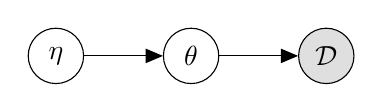
\begin{tikzpicture}
    \node[latent] (e) {$\boldsymbol{\eta}$};
    \node[latent, right=of e] (t) {$\boldsymbol{\theta}$};
    \node[obs, right=of t] (d) {$\mathcal{D}$};
    \edge {e} {t}
    \edge{t} {d}
\end{tikzpicture}
\end{figure*}

\item[Uninformative Priors:] An uninformative prior is a distribution which does not favor any outcome, and thereby does not incorporate any prior knowledge. It is like saying one simply does not know what to believe.
\item[Empirical Bayes:] The priors can be estimated from the data, resulting in the so-called Empirical Bayes method. The parameters of the prior can be found by maximizing the conditional likelihood. %TODO: cite
\end{description}


\section{Stochastic Modelling}

\subsection{Markov Chains}
A Markov Chain is a chain of events, where the outcome of the next event only depends on the current state. All information needed to predict the future is contained in the current state. This property is called the \textit{Markov Property} and is expressed in \cref{eq:theory_markov_property}.

\begin{equation}\label{eq:theory_markov_property}
p(\mathbf{X}_{t+1} | \mathbf{X}_t,  \mathbf{X}_{0:t-1}) = p(\mathbf{X}_{t+1} | \mathbf{X}_t)  \quad \forall t \in [1, \infty)
\end{equation}

\subsubsection{Stationary Distribution}
As time moves on, some states will be visited more frequently than others. This long-running distribution of states is called the \textit{stationary distribution} of the Markov Chain. If $\mathbf{P}$ is the transition probability matrix for a discrete Markov chain, then $\boldsymbol{\pi}$ is the stationary distribution if 
\begin{equation}\label{eq:markov_stationary}
    \boldsymbol{\pi} = \boldsymbol{\pi} \mathbf{P}
\end{equation}

The stationary distribution may not be unique, and whether a unique stationary distribution exists, depends on how the Markov Chain behaves. Further details on stationary distributions are outside the scope of this thesis. 



\section{Probabilistic Graphical Models}
\textit{\acrfull{pgm}}, often called Bayesian Networks, allows for efficient factorization of the joint distribution by assuming conditional independence, as defined in \cref{eq:conditional_independence}, between variables. \acrshort{pgm}'s are graphs, where nodes represent random variables and edges represents statistical dependence between the variables. By utilizing the independence assumptions in the graphs, the computational complexity can be drastically reduced \cite{murphy}.

\subsection{\acrfull{dgm}}
\acrshort{dgm}'s are perhaps the simplest type of \acrshort{pgm} and is based on \textbf{Directed Acyclic Graphs} (DAG). It is a graph structure which do not allow cycles and all edges are directed. The flow of information is explicitly modeled in the direction on the edges. \acrshort{dgm}'s are well-suited for modelling causal relationships and when the flow of information is clearly directed. An example can be the relationship between the state of a physical system and a sensor. The system affects the sensor, but the sensor does not affect the system. For the \acrshort{dgm} in \cref{fig:dgm}, the variables $B$ and $C$ are conditionally independent given $A$, i.e. $B \perp C | \; A$. However, knowing $D$ restricts $C$ and $B$, i.e. $B \not\perp C | \; D$. This all comes directly from inspecting the graph. 

\acrshort{dgm} allows for straight-forward factorization of the joint-distribution 
\begin{equation}\label{eq:dgm_factorization}
    p(\mathbf{x}) = \prod_{v \in \mathcal{V}}p(v | \mathbf{pa}(v))
\end{equation}
where $\mathcal{V}$ is all the nodes in the graph and $\mathbf{pa}(v)$ is the parent's for node $v$. 

\subsection{\acrfull{mrf}} \label{sec:mrf}

\acrshort{mrf}'s are undirected graphical models, and offers a more general specification of independence assumptions. They are in some domains, such as relational or spatial data , more natural than \acrshort{dgm}'s as they are symmetric, i.e. the information flows both ways \cite{murphy}. The \acrshort{mrf} in \cref{fig:mrf} shows that $B$ and $C$ is only independent if both $A$ and $D$ is observed, i.e. $B \perp C | \; A, D$. The important thing to notice is that the \acrshort{mrf} makes vastly different assumptions than the \acrshort{dgm}, even though the structure is similar.

By the \textbf{Hammersley-Clifford Theorem} \cite[p.~ 668]{murphy}, the joint distribution of \acrshort{mrf} models can be factorized on the form
\begin{equation}
    p(\mathbf{x}) =\frac{1}{Z} \prod_{c \in \mathcal{C}} \psi_c(\mathbf{x}_c)
\end{equation}
where is $\mathcal{C}$ is the set of all \textit{maximal cliques}, i.e. largest, fully connected sub graphs. All variables in a maximal clique is therefore dependent on each other. $\psi_c(\cdot)$ is the \textit{(factor) potential function} for the nodes in the clique $c$, and determines the strength of the interaction between the variables $\bf{x}_c$. The \textit{(factor) partition function}
\begin{equation}
    Z = \int_\mathbf{x} (\prod_{c \in \mathcal{C}} \psi_c(\mathbf{x}_c)) d \mathbf{x}
\end{equation}
is a normalization constant so that $p(\mathbf{x}) \in [0, 1]$. The potential functions $\psi_c(\cdot)$ can therefore be arbitrary non-negative functions. 

\acrshort{dgm}'s can be converted into \acrshort{mrf}'s through \textit{\gls{moralization}}. \Gls{moralization} is performed by making all edges undirected and add new edges between variables sharing a child. Some independence information is lost in the process, but it represent the same factorization of the joint distribution. The computational complexity of inference on \acrshort{dgm}s and \acrshort{mrf}s are, generally speaking, the same  \cite{murphy}. Inference methods for \acrshort{mrf}'s can therefore also be used on \acrshort{dgm}'s by first moralizing.


\subsection{Factor Graphs}
Factor Graphs unifies the concept of directed (\acrshort{dgm}) and undirected graphical models (\acrshort{mrf}). A factor graph is an undirected bipartite graph. Bipartite graphs are graphs with two different types of nodes, factors and variables. All variables are represented by round nodes and all factors are square nodes. Each factor is connected to all variables it references through undirected edges. Both \acrshort{mrf}'s and \acrshort{dgm}'s can be converted to factor graphs. Factor graphs is not really intended for modelling independence, but rather visualize how the joint distribution can be factorized to allow for efficient computations. \cref{fig:factor} shows a factor graph for the \acrshort{mrf} in \cref{fig:mrf}.

For generative models, an extension to factor graph notation is proposed in \cite{dietz} to allow for a more intuitive reasoning about the model. The directed edges in \cref{fig:factor_directed} contains additional information about how realizations of the random variables are generated, similar to the \acrshort{dgm} in \cref{fig:dgm}. The factors can the be viewed intuitively as generative processes, with input and output variables. It otherwise contain the exact same functional representation as the normal factor graph in \cref{fig:factor}. 

\begin{figure}[h]
\centering
\begin{subfigure}{0.49\textwidth}
\centering
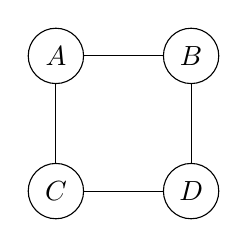
\begin{tikzpicture}
    \node[latent] (A) {$A$};
    \node[latent, right=of A] (B) {$B$};
    \node[latent, below=of A] (C) {$C$};
    \node[latent, below=of B] (D) {$D$};
    \edge[-] {A} {B};
    \edge[-] {A} {C};
    \edge[-] {C} {D}
    \edge[-] {B} {D}
\end{tikzpicture}
\caption{\acrfull{mrf}}
\label{fig:mrf}
\end{subfigure}
\begin{subfigure}{0.49\textwidth}
\centering
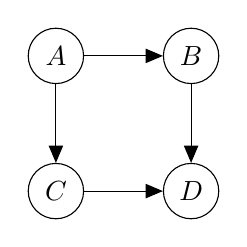
\begin{tikzpicture}
    \node[latent] (A) {$A$};
    \node[latent, right=of A] (B) {$B$};
    \node[latent, below=of A] (C) {$C$};
    \node[latent, below=of B] (D) {$D$};
    \edge {A} {B};
    \edge {A} {C};
    \edge {C} {D}
    \edge {B} {D}
\end{tikzpicture}
\caption{\acrfull{dgm}}
\label{fig:dgm}
\end{subfigure}
\begin{subfigure}{0.49\textwidth}
\centering
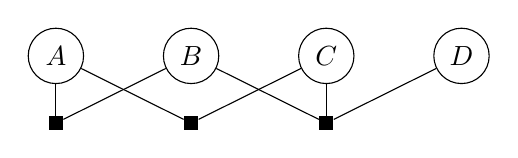
\begin{tikzpicture}
    \node[latent] (A) {$A$};
    \node[latent, right=of A] (B) {$B$};
    \node[latent, right=of B] (C) {$C$};
    \node[latent, right=of C] (D) {$D$};
    \factor[below=of A] {ba-factor} {} {} {};
    \factor[below=of B] {ca-factor} {} {} {};
    \factor[below=of C] {dbc-factor} {} {} {};
    \factoredge{A, B}{ba-factor}{}
    \factoredge{A, C}{ca-factor}{}
    \factoredge{B, C, D}{dbc-factor}{}
\end{tikzpicture}
\caption{Factor Graph}
\label{fig:factor}
\end{subfigure}
\begin{subfigure}{0.49\textwidth}
\centering
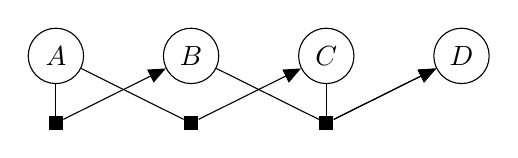
\begin{tikzpicture}
    \node[latent] (A) {$A$};
    \node[latent, right=of A] (B) {$B$};
    \node[latent, right=of B] (C) {$C$};
    \node[latent, right=of C] (D) {$D$};
    \factor[below=of A] {ba-factor} {} {} {};
    \factor[below=of B] {ca-factor} {} {} {};
    \factor[below=of C] {dbc-factor} {} {} {};
    \factoredge{A}{ba-factor}{B}
    \factoredge{A}{ca-factor}{C}
    \factoredge{B}{dbc-factor}{D}
    \factoredge{C}{dbc-factor}{D}
\end{tikzpicture}
\caption{Factor Graph for generative model}
\label{fig:factor_directed}
\end{subfigure}

\caption{\acrshort{pgm} representations of a probabilistic models with $4$ variables.}
\end{figure}

\section{Probability Distributions}

\subsection{Transformations}
TODO: Add equation

\subsection{Conjugate Priors}\label{sec:theory_conjugate_priors}
If the posterior distribution is in the same family as the prior, then the posterior is called the \textit{conjugate distribution} and the prior is called the \textit{conjugate prior}. Using conjugate priors in Bayesian Statistics, allows for analytically tractable inference as the posterior becomes a well known probability distribution. \cref{table:conjugate_priors} summarizes the conjugate priors for a few common distribution.


\begin{table}[h]
\begin{tabular}{lllll}
\hline
\multicolumn{1}{|l|}{\textbf{Distribution}} & \multicolumn{1}{l|}{\textbf{1st Parent}}        & \multicolumn{1}{l|}{\textbf{Conjugate}} & \multicolumn{1}{l|}{\textbf{2nd Parent}} & \multicolumn{1}{l|}{\textbf{Conjugate}} \\ \hline
\multicolumn{1}{|l|}{Gaussian}              & \multicolumn{1}{l|}{mean $\mu$}                 & \multicolumn{1}{l|}{Gaussian}           & \multicolumn{1}{l|}{precision $\gamma$}  & \multicolumn{1}{l|}{Gamma}              \\ \hline
\multicolumn{1}{|l|}{Gamma}                 & \multicolumn{1}{l|}{shape $\alpha$}             & \multicolumn{1}{l|}{none}               & \multicolumn{1}{l|}{scale $b$}           & \multicolumn{1}{l|}{Gamma}              \\ \hline
\multicolumn{1}{|l|}{Discrete}              & \multicolumn{1}{l|}{probabilities $\mathbf{p}$} & \multicolumn{1}{l|}{Dirichlet}          & \multicolumn{1}{l|}{parents $\{x_i\}$}   & \multicolumn{1}{l|}{Discrete}           \\ \hline
\multicolumn{1}{|l|}{Dirichlet}             & \multicolumn{1}{l|}{pseudo-counts $\bf a$}      & \multicolumn{1}{l|}{none}               & \multicolumn{1}{l|}{}                    & \multicolumn{1}{l|}{}                   \\ \hline
\multicolumn{1}{|l|}{Exponential}           & \multicolumn{1}{l|}{scale $\alpha$}             & \multicolumn{1}{l|}{Gamma}              & \multicolumn{1}{l|}{}                    & \multicolumn{1}{l|}{}                   \\ \hline
\multicolumn{1}{|l|}{Poisson}               & \multicolumn{1}{l|}{mean $\lambda$}             & \multicolumn{1}{l|}{Gamma}              & \multicolumn{1}{l|}{}                    & \multicolumn{1}{l|}{}                   \\ \hline
\end{tabular}
\caption{Table of conjugate priors for common, standard distributions. For cells with \textit{none}, there exist no standard distribution as a conjugate prior. \cite[p.~676]{winnbishop}}
\label{table:conjugate_priors}
\end{table}


\subsection{Beta \& Dirichlet Distributions}
The Beta distribution is a distribution with support between $0$ and $1$, and is therefore well suited to model probabilities. The Dirichlet distribution is a multivariate generalization of the Beta distribution. 
\subsection{Binomial \& Multinomial Distributions}
\subsection{Dirichlet-Multinomial Distribution}
\subsection{Bernouilli \& Categorial Distributions}
\subsection{Normal Distribution}
\subsection{The Exponential Family}
The Exponential Family is a family of distribution for which the \acrshort{pdf} or \acrshort{pmf} can be expressed on the from
\begin{equation}
    p(\mathbf{x} | \boldsymbol{\theta}) = h(\mathbf{x}) \exp[\eta(\boldsymbol{\theta}) T(\mathbf{x}) - A(\boldsymbol{\theta})]
\end{equation}
All the distributions mentioned so far are part of the Exponential Family. Distributions in the exponential family always have conjugate priors, however they may not be standard, well-known distributions. %TODO CITE

\chapter{Non-parametric trajectories using Gaussian Process}\label{chap:impl}
Predicting vessel trajectories can be parametrized in multiple ways. The simplest parametrization would be to directly model the trajectory $f(t)$ from observed data. Another approach is to rather learn a vector-field from AIS gradients, and use the vector field as variable input to a linear model. The vector-field can then be though of as forces, or flows, pushing the vessel in the direction of historical AIS data. A simple Kalman-filter predict step can then be used to simulate the movement for any vessel placed in the vector-field. 


\section{Non-parametric dynamic system using AIS tracking data}
The trajectory $\mathcal{T}$ can be expressed using the dynamical system model $\dot{\boldsymbol{x}} = f(\boldsymbol{x})$
\begin{subequations}
\begin{align}
    \boldsymbol{x}(t) &= \boldsymbol{x}(0) + \int_0^t \vec{f}(\boldsymbol{x}(\tau)) d\tau \\
    \mathcal{T}(t) &= \boldsymbol{x}(t) + \epsilon, \quad \epsilon \sim \mathcal{N}(0, \sigma^2)
\end{align}
\end{subequations}

The function $\vec{f}(\cdot): \mathcal{R}^2 \to \mathcal{R}^2$ denotes the vector field describing the forces acting on a vessel. Normally this function is parametrized explicitly and the solution is solved either analytically or numerically depending on the complexity of the model. However, in the case of long-term prediction, the dynamics $\vec{f}(\cdot)$ is unknown and is unlikely stationary. Instead, the goal of this chapter is to use a \acrshort{gp} to create a non-parametric representation of the dynamics $\vec{f}(\cdot)$ by learning from historical trajectories of other vessels.

\begin{equation}\label{eq:gp_vec_field}
    f(\boldsymbol{x}) = \begin{bmatrix} f_x (\boldsymbol{x})\\ f_y (\boldsymbol{x})\end{bmatrix} \sim \text{GP} \big(\begin{bmatrix} m_x(\boldsymbol{x})\\m_y(\boldsymbol{x})\end{bmatrix}, \ \begin{bmatrix}
    K_{xx}(\boldsymbol{x}, \boldsymbol{x}') & K_{xy}(\boldsymbol{x}, \boldsymbol{x}') \\ K_{xy}(\boldsymbol{x}, \boldsymbol{x}')^\intercal & K_{yy}(\boldsymbol{x}, \boldsymbol{x}')
    \end{bmatrix}\big) 
\end{equation}

The benefits of this formulation include:
\begin{description}
    \item[Easy incorporation of existing data] The model can easily be trained on partial data. Only the gradients of any historical trajectories are really needed.
    \item[Few constraining assumptions] The dynamical model is not constrained by any specific parametrization, while still allows prior knowledge such as smoothness to be incorporated into the model.
    \item[Uncertainty] The model can express uncertain when the availability of examples are sparse. 
\end{description}

\cite{heinonen2018learningode} use a similar formulation to infer arbitrary, non-linear ODE models from sparse data and predict the dynamics far into the future. 

\section{Learning trajectories directly from data (?)}
\section{Branching Trajectories}
\subsection{Mixture of Gaussian Process Experts}


\chapter{Statistical Testing}\label{chap:stat_testing}
Inspired by \cite{hexeberg}, the performance of the proposed models will be compared on straight-line and curved trajectories independently.

\section{Method}
\subsection{Trajectory Error}
The trajectory error is found by comparing the predicted position with the ground truth. As the predicted trajectory is simulated in discrete time, the points with the closest timestamps are used for comparison. With $\Delta T = 10\text{ seconds}$, the maximum error in time is $\frac{\Delta T}{2} = 5 \text{ seconds}$, which is considered to be acceptable considering the time-horizon of between $15$ and $30$ minutes.
\subsection{Path Error}
The path error is defined as the closest point in the predicted trajectory to each point in the ground truth, under the constraint that the corresponding predicted timestamps must be monotonically increasing. In other words, the path cannot move backward in time. Linear interpolation is used to get the path error at fixed timestamps to simplify the comparison.

\subsection{Normalized Estimation Error Squared}
In order for the uncertainty estimates to provide any value, it is important that the predictions are consistent. In this context, the term consistency is borrowed from the term \textit{filter consistency} used when tuning Kalman filters \cite{sensorfusjon}. The idea is that prediction errors, on average, should scale with the state covariance. In other words, the model should not place a lot of confidence in a prediction that is wrong while being highly confident when a prediction is correct. Consistency can also be interpreted using a frequentistic interpretation of probability, where after many predictions, the state uncertainty should reflect the actual error rate.

The \textit{\acrfull{nees}} is a metric that can be used to quantify consistency and is given by
\begin{equation}
    \text{NEES} = (\boldsymbol{x} - \hat{\boldsymbol{x}})^\intercal \boldsymbol{P}^{-1} (\boldsymbol{x} - \hat{\boldsymbol{x}})
\end{equation}

Assuming the prediction error follows a Gaussian distribution, the \acrshort{nees} follows a Chi-Squared distribution which can be used to form a confidence interval. Comparing the prediction errors with this confidence interval can then be used to get a sense of whether the estimated state uncertainty is consistent with the actual error rate.

\subsection{Interpolation}
Linear interpolation is used to compare the metrics at fixed timestamps between samples. The error for short trajectories is not extrapolated.

\subsection{Baseline - Constant Velocity Model}
As a basis of comparison, the \textit{\acrfull{cvm}} method is used as a baseline. The model use the initial \acrshort{cog} and \acrshort{sog} to predict a straight line, where the vessel is assumed to keep a constant velocity and heading.

\subsection{Sanitizing the dataset for a given test trajectory}
Due to the way trajectories are generated from the \acrshort{ais} dataset, there will be large overlaps between trajectories. Dividing the trajectories into a train and test is insufficient, as parts of a test trajectory might also exist in the training set. Instead, the full dataset is available for training, but all trajectories with identical MMSI and date as the test trajectory are removed. The date requirement ensures that trajectories for the same vessel on any other day can be used for training.

\subsection{Straigth-line trajectories}
The GP-EKF is first compared to the \acrshort{cvm} on simple straight-line trajectories. The GP-EKF should ideally perform identically or better than the \acrshort{cvm}.
The statistics are based on $350$ randomly sampled trajectories without replacement that satisfy the following requirements:
\begin{enumerate}
    \item The sum of subsequent changes in \acrshort{cog} must be less than $30$ degrees, i.e. $\sum_i |(\mathcal{X}_{t+1} - \mathcal{X}_t)| \leq 30^\circ$. This requirement ensures a straight-line trajectory.
    \item There must be sufficient data available for training in the neighborhood around the initial starting point, with similar initial heading and speed. After sanitizing the dataset and removing irrelevant trajectories, at least $3$ trajectories need to be available for training.
    \item The overall duration of the trajectories must be between $15$ and $30$ minutes.
\end{enumerate}




\subsection{Curved Trajectories}
The GP-EKF is then compared to the \acrshort{cvm} on curved trajectories. The GP-EKF should ideally perform drastically better than the \acrshort{cvm}.
The statistics are based on $350$ randomly sampled trajectories that satisfy the following requirements:
\begin{enumerate}
    \item The sum of subsequent changes in \acrshort{cog} must be greater than $40$ degrees, i.e. $\sum_i |(\mathcal{X}_{t+1} - \mathcal{X}_t)| \geq 40^\circ$. This requirement ensures a straight-line trajectory.
    \item There must be sufficient data available for training in the neighborhood around the initial starting point, with similar initial heading and speed. After sanitizing the dataset and removing irrelevant trajectories, at least $3$ trajectories need to be available for training.
    \item The overall duration of the trajectories must be between $15$ and $30$ minutes.
\end{enumerate}

\section{Results}
The results for straight-line and curved trajectories are available in \cref{table:stats_straight_line_error} and \cref{table:stats_curved_error} respectively. \todo[]{add examples in appendix?}. As expected, the \acrshort{cvm} method performs well on the straight-line trajectories, while struggles on the curved trajectories.
\begin{table}
    \begin{subtable}{\textwidth}
        \makebox[\textwidth][c]{
            \begin{tabular}{lllrrrrr}
                \toprule
                        &                & Time [Minutes]    & 5   & 10   & 15   & 20   & 25   \\
                Summary & Method         & Training Source   &     &      &      &      &      \\
                \midrule
                Mean    & CVM            & COG/SOG from AIS  & 674 & 1347 & 2024 & 2332 & 2272 \\
                        & Direct GP      & Position          & 969 & 1319 & 1838 & 2557 & 2845 \\
                        & GP-EKF         & COG/SOG from AIS  & 590 & 1169 & 1678 & 1883 & 2318 \\
                        &                & Finite Difference & 562 & 1078 & 1645 & 2400 & 2560 \\
                        & GP-EKF w/ PDAF & COG/SOG from AIS  & 596 & 1149 & 1618 & 1848 & 2207 \\
                        &                & Finite Difference & 568 & 1059 & 1603 & 2323 & 2448 \\
                \midrule
                Median  & CVM            & COG/SOG from AIS  & 481 & 968  & 1538 & 1863 & 2073 \\
                        & Direct GP      & Position          & 549 & 892  & 1295 & 1896 & 2529 \\
                        & GP-EKF         & COG/SOG from AIS  & 445 & 888  & 1258 & 1373 & 2402 \\
                        &                & Finite Difference & 418 & 682  & 1140 & 1591 & 1841 \\
                        & GP-EKF w/ PDAF & COG/SOG from AIS  & 443 & 866  & 1203 & 1353 & 2367 \\
                        &                & Finite Difference & 427 & 683  & 1108 & 1503 & 1736 \\
                \bottomrule
            \end{tabular}
        }
        \caption{Trajectory errors in meters}
        \label{table:stats_straight_traj_err}
        \vspace*{0.5cm}
    \end{subtable}
    \begin{subtable}{\textwidth}
        \makebox[\textwidth][c]{
            \begin{tabular}{lllrrrrr}
                \toprule
                        &                & Time [Minutes]    & 5   & 10  & 15   & 20   & 25   \\
                Summary & Method         & Training Source   &     &     &      &      &      \\
                \midrule
                Mean    & CVM            & COG/SOG from AIS  & 142 & 497 & 1144 & 1550 & 2033 \\
                        & Direct GP      & Position          & 487 & 534 & 806  & 1412 & 2195 \\
                        & GP-EKF         & COG/SOG from AIS  & 218 & 483 & 949  & 1183 & 1408 \\
                        &                & Finite Difference & 229 & 460 & 745  & 1249 & 1042 \\
                        & GP-EKF w/ PDAF & COG/SOG from AIS  & 209 & 442 & 867  & 1118 & 1298 \\
                        &                & Finite Difference & 222 & 428 & 692  & 1173 & 957  \\
                \midrule
                Median  & CVM            & COG/SOG from AIS  & 70  & 262 & 703  & 1206 & 1971 \\
                        & Direct GP      & Position          & 181 & 310 & 429  & 782  & 2186 \\
                        & GP-EKF         & COG/SOG from AIS  & 142 & 310 & 602  & 785  & 959  \\
                        &                & Finite Difference & 143 & 277 & 375  & 700  & 743  \\
                        & GP-EKF w/ PDAF & COG/SOG from AIS  & 145 & 284 & 515  & 742  & 841  \\
                        &                & Finite Difference & 146 & 250 & 357  & 646  & 761  \\
                \bottomrule
            \end{tabular}
        }
        \caption{Path error in meters}
        \label{table:stats_straight_path_err}
    \end{subtable}
    \caption{Error summary for $350$ straight-line trajectories. Mean and median summary statistics are calculated for the trajectory and path error at fixed timestamps. Linear interpolation is used between samples. Errors for short trajectories are not extrapolated, and therefore not included in the $20$ and $25$ minute bins.}
    \label{table:stats_straight_line_error}
\end{table}

\begin{table}
    \begin{subtable}{\textwidth}
        \makebox[\textwidth][c]{
            \begin{tabular}{lllrrrrr}
                \toprule
                        &                & Time [Minutes]    & 5    & 10   & 15   & 20    & 25    \\
                Summary & Method         & Training Source   &      &      &      &       &       \\
                \midrule
                Mean    & CVM            & COG/SOG from AIS  & 1282 & 3238 & 6127 & 10066 & 14604 \\
                        & Direct GP      & Position          & 490  & 736  & 889  & 893   & 979   \\
                        & GP-EKF         & COG/SOG from AIS  & 787  & 1614 & 2331 & 2909  & 3520  \\
                        &                & Finite Difference & 709  & 1392 & 1835 & 2242  & 2380  \\
                        & GP-EKF w/ PDAF & COG/SOG from AIS  & 722  & 1449 & 1986 & 2290  & 2310  \\
                        &                & Finite Difference & 724  & 1355 & 1752 & 2098  & 2233  \\
                \midrule
                Median  & CVM            & COG/SOG from AIS  & 875  & 2605 & 5419 & 10325 & 15008 \\
                        & Direct GP      & Position          & 233  & 381  & 479  & 531   & 644   \\
                        & GP-EKF         & COG/SOG from AIS  & 614  & 1258 & 1949 & 2521  & 3603  \\
                        &                & Finite Difference & 512  & 982  & 1582 & 2049  & 2162  \\
                        & GP-EKF w/ PDAF & COG/SOG from AIS  & 525  & 1101 & 1461 & 1457  & 1829  \\
                        &                & Finite Difference & 534  & 922  & 1527 & 1890  & 2168  \\
                \bottomrule
            \end{tabular}
        }
        \caption{Trajectory Error in meters}
        \label{table:stats_curved_traj_err}
        \vspace*{0.5cm}
    \end{subtable}
    \begin{subtable}{\textwidth}
        \makebox[\textwidth][c]{
            \begin{tabular}{lllrrrrr}
                \toprule
                        &                & Time [Minutes]    & 5   & 10   & 15   & 20   & 25   \\
                Summary & Method         & Training Source   &     &      &      &      &      \\
                \midrule
                Mean    & CVM            & COG/SOG from AIS  & 484 & 1383 & 2793 & 4494 & 6105 \\
                        & Direct GP      & Position          & 323 & 409  & 456  & 514  & 662  \\
                        & GP-EKF         & COG/SOG from AIS  & 267 & 671  & 1383 & 2046 & 2870 \\
                        &                & Finite Difference & 400 & 615  & 742  & 723  & 565  \\
                        & GP-EKF w/ PDAF & COG/SOG from AIS  & 259 & 565  & 1054 & 1466 & 1678 \\
                        &                & Finite Difference & 412 & 594  & 704  & 682  & 538  \\
                \midrule
                Median  & CVM            & COG/SOG from AIS  & 188 & 776  & 1867 & 3671 & 6797 \\
                        & Direct GP      & Position          & 92  & 161  & 180  & 192  & 276  \\
                        & GP-EKF         & COG/SOG from AIS  & 114 & 323  & 863  & 1340 & 2555 \\
                        &                & Finite Difference & 227 & 398  & 481  & 437  & 344  \\
                        & GP-EKF w/ PDAF & COG/SOG from AIS  & 130 & 264  & 512  & 789  & 916  \\
                        &                & Finite Difference & 274 & 389  & 458  & 403  & 363  \\
                \bottomrule
            \end{tabular}
        }
        \caption{Path error in meters}
        \label{table:stats_curved_path_err}
    \end{subtable}
    \caption{Error summary for $350$ curved trajectories. Mean and median summary statistics are calculated for the trajectory and path error at fixed timestamps. Linear interpolation is used between samples. Errors for short trajectories are not extrapolated, and therefore not included in the $20$ and $25$ minute bins.}
    \label{table:stats_curved_error}
\end{table}


\subsection{Comparing Direct GP to CVM}
\begin{figure}[h]
    \centering
    \makebox[\textwidth][c]{
        \begin{subfigure}{0.65\textwidth}
            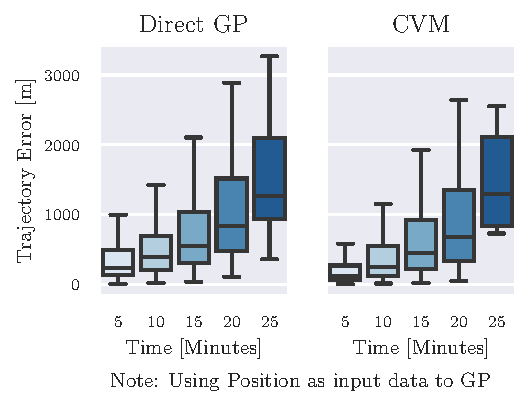
\includegraphics[width=\textwidth]{figures/straight_line_stats/gp_vs_cvm_1.pdf}
            \caption{Straight-Line Trajectories}
        \end{subfigure}
        \begin{subfigure}{0.65\textwidth}
            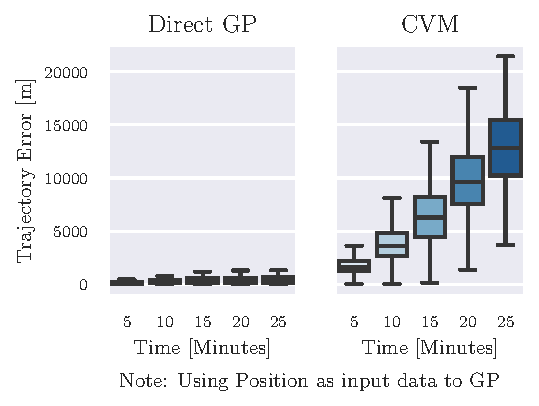
\includegraphics[width=\textwidth]{figures/curved_line_stats/gp_vs_cvm_1.pdf}
            \caption{Curved Trajectories}
        \end{subfigure}
    }
    \caption{GP-EKF compared to the CVM method on $350$ random trajectories. As expected, the \acrshort{cvm} yields large trajectory errors on curved trajectories. The GP-EKF performs consistently better, with lower median error as well as lower spread. However, on straight-line trajectories, the methods behave comparably.}
    \label{fig:stats_curved_posgp_cvm}
\end{figure}
The Direct GP approach performs slightly worse than the \acrshort{cvm} on straight-line trajectories, while it performs significantly better on curved trajectories, with overall lower spread and median trajectory error as depicted in \cref{fig:stats_curved_gp_ekf_cvm}.

\subsection{Comparing GP-EKF to CVM}
\begin{figure}[h]
    \centering
    \makebox[\textwidth][c]{
        \begin{subfigure}{0.65\textwidth}
            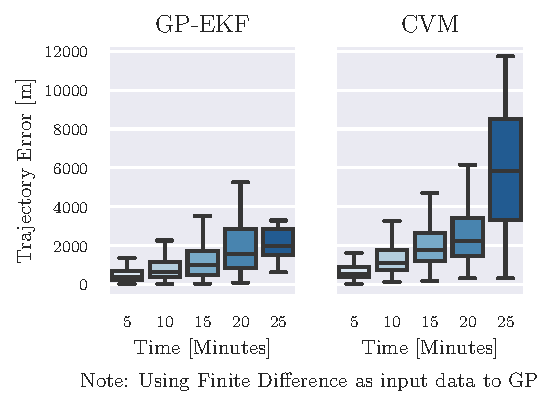
\includegraphics[width=\textwidth]{figures/straight_line_stats/gp_vs_cvm_3.pdf}
            \caption{Straight-Line Trajectories}
        \end{subfigure}
        \begin{subfigure}{0.65\textwidth}
            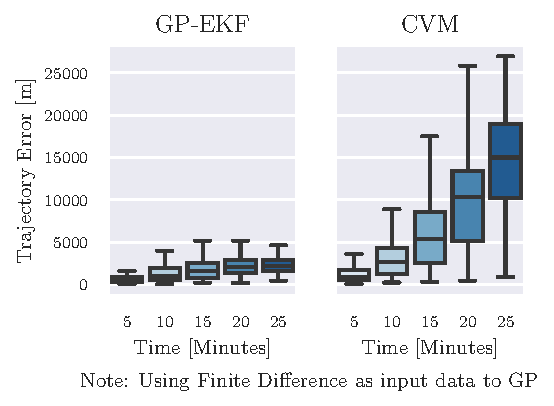
\includegraphics[width=\textwidth]{figures/curved_line_stats/gp_vs_cvm_3.pdf}
            \caption{Curved Trajectories}
        \end{subfigure}
    }
    \caption{GP-EKF compared to the CVM method on $350$ random trajectories. As expected, the \acrshort{cvm} yields large trajectory errors on curved trajectories. The GP-EKF performs consistently better, with lower median error as well as lower spread. However, on straight-line trajectories, the methods behave comparably.}
    \label{fig:stats_curved_gp_ekf_cvm}
\end{figure}
The GP-EKF approach performs significantly better than the \acrshort{cvm} on curved trajectories, with overall lower spread and median trajectory error as depicted in \cref{fig:stats_curved_gp_ekf_cvm}.

\subsection{Effect of the PDAF update}
\begin{figure}
    \centering
    \makebox[\textwidth][c]{
        \begin{subfigure}{0.65\textwidth}
            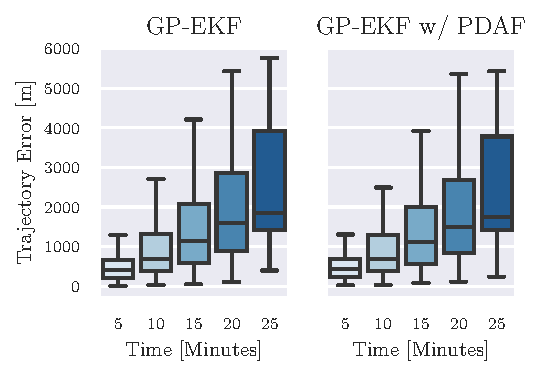
\includegraphics[width=\textwidth]{figures/straight_line_stats/gp_vs_pdaf.pdf}
            \caption{Straight-Line Trajectories}
        \end{subfigure}
        \begin{subfigure}{0.65\textwidth}
            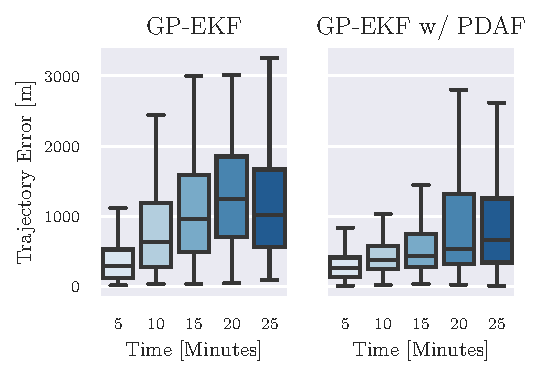
\includegraphics[width=\textwidth]{figures/curved_line_stats/gp_vs_pdaf.pdf}
            \caption{Curved Trajectories}
        \end{subfigure}
    }
    \caption{GP-EKF with and without PDAF on curved trajectories for $350$ trajectories. While there are some slight differences, the \acrshort{pdaf} does not appear to have any considerable effect on the trajectory errors.}
    \label{fig:stats_gp_ekf_with_or_without_pdaf}
\end{figure}

When comparing the performance of GP-EKF with and without the update step in \cref{fig:stats_gp_ekf_with_or_without_pdaf}, there seems to be little actual gain from the added complexity of \acrshort{pdaf}.


\subsection{Finite Difference vs. COG/SOG from AIS}
A key design choice for the GP-EKF is which data source to use for training. The model can either be trained using the \acrshort{cog} and \acrshort{sog} values contained in the \acrshort{ais} samples or by calculating numerical derivatives of the position through a finite-difference approach. Comparing trajectory error for both approaches on the same test set favors the finite-difference approach, as seen in \cref{fig:stats_curved_gp_ekf_fd_vs_cog}. The finite difference approach performs consistently better, with lower median error and less spread. However, by ignoring the time component, looking at the path errors in \cref{table:stats_curved_path_err} supports the opposite, where the path errors are lower for the \acrshort{cog}/\acrshort{sog} approach. This may indicate that the issue is due to imprecise velocity estimates from the \acrshort{sog} while using the course from the \acrshort{cog} works well.
\begin{figure}
    \centering
    \makebox[\textwidth][c]{
        \begin{subfigure}{0.65\textwidth}
            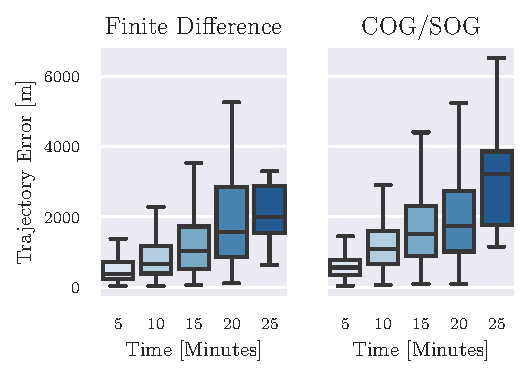
\includegraphics{figures/straight_line_stats/gp_cog_vs_fd.pdf}
            \caption{Straight-Line Trajectory}
        \end{subfigure}
        \begin{subfigure}{0.65\textwidth}
            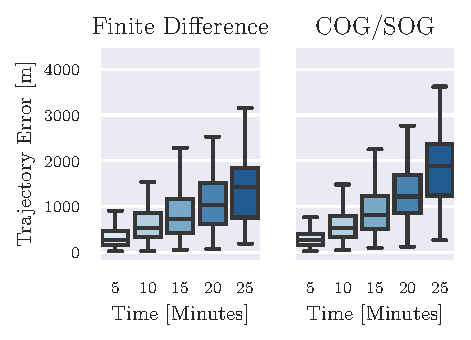
\includegraphics{figures/curved_line_stats/gp_cog_vs_fd.pdf}
            \caption{Curved Trajectory}
        \end{subfigure}
    }
    \caption{GP-EKF using finite differences and the \acrshort{cog} and \acrshort{sog} from the AIS dataset on $350$ trajectories. The finite differences approach performs consistently better, with lower median error and spread.}
    \label{fig:stats_curved_gp_ekf_fd_vs_cog}
\end{figure}


\section{Consistency}
\begin{figure}[h]
    \centering
    \makebox[\textwidth][c]{
        \begin{subfigure}{0.65\textwidth}
            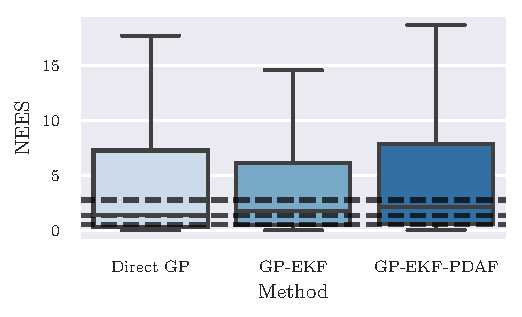
\includegraphics{figures/straight_line_stats/nees.pdf}
            \caption{Straight-Line Trajectory}
        \end{subfigure}
        \begin{subfigure}{0.65\textwidth}
            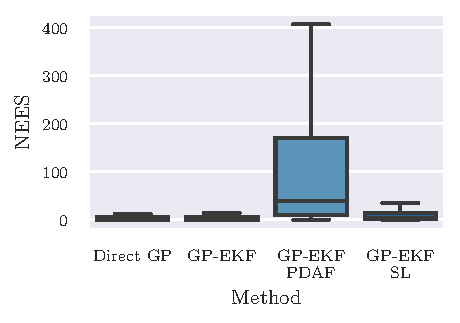
\includegraphics{figures/curved_line_stats/nees.pdf}
            \caption{Curved Trajectory}
        \end{subfigure}
    }
    \begin{subfigure}{0.65\textwidth}
        \centering
        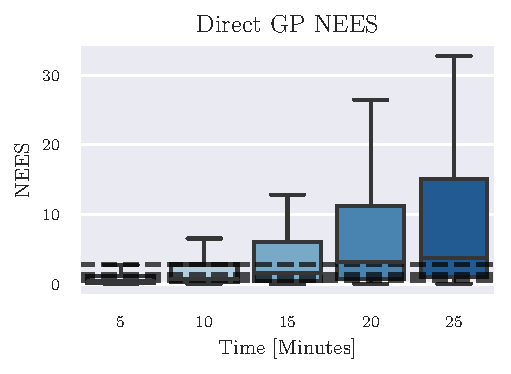
\includegraphics{figures/curved_line_stats/direct_gp_nees.pdf}
        \caption{Direct GP NEES for curved trajectories}
        \label{fig:stats_curved_nees_direct}
    \end{subfigure}
    \caption{Boxplot of the \acrshort{nees} on straight-line and curved trajectories for each method. The dotted lines shows the theoritical quartiles ($25\%$, $50\%$ and $75\%$) for the $\mathcal{X}^2$ distribution as a comparison.}.
    \label{fig:stats_curved_nees}
\end{figure}
The estimated quartiles \acrshort{nees} for straight-line and curved trajectories is displayed for each method in \cref{fig:stats_curved_nees}.

On straight-line trajectories, the $25\%$ and $50\%$ quartiles correspond well with the theoretical values for the $\mathcal{X}^2$ distribution for all methods. The \acrshort{pdaf} update step does, however, reduce the predicted uncertainty, leading to increased overconfidence. In addition, the estimated \acrshort{nees} distribution has a much fatter right-tail than the theoretical $\mathcal{X}^2$ distribution, leading to an estimated $75\%$ quartile far outside the theoretical values.

On curved trajectories, the GP-EKF with and without PDAF is consistently overconfident. The theoretical quartiles are not plotted due to the large y-axis. The direct \acrshort{gp} approach performs significantly better, which is why a separate plot in \cref{fig:stats_curved_nees_direct} is added to compare it to theoretical quartiles. 





\chapter{Discussion}

All of the methods described in this thesis so far have their strong advantages and disadvantages. 

\section{When all variables are discrete}
In the case of \acrshort{pgm}'s with only discrete variables, exact inference methods are often applicable. The challenges of Bayesian inference in such networks usually boils down to computational complexity when the number of variables increases. Exact methods such as \acrshort{bp} are in most cases the most appropriate choice, though some structures (in the case of loops) cannot guarantee an optimal solution. 

\section{When some variables are continuous}
When some variables are continuous, the problem usually gets a bit more complicated. If all parent-child can be expressed using conjugate-priors, exact methods can still be used. However, requiring the use of only conjugate-priors may in many cases be too restrictive as it limits the ability to express intuitive understanding of the data-generating process. 

The most straight-forward approach will be to use \acrshort{mcmc} methods, due to their simplicity. These methods allow sampling from arbitrarily complex models as long as the target probability can be evaluated. It can in most cases provide asymptotic guarantees that the samples is from the true posterior distribution, though only given a very large amount of samples. How many samples that are considered "enough" is difficult to say, and it usually require manual interpretations of the results in order to verify convergence. Using \acrshort{mcmc} in autonomous systems may therefore be challenging unless the model is sufficiently simple, in which case other methods may still be preferable. Due to the random nature of sampling methods, \acrshort{mcmc} is likely a poor choice for problems where deterministic behaviour is valued.



Though it requires more work, \acrshort{vi} will in many cases be a better option. By posing the problem as a optimization problem rather than relying on sampling, variational inference can give deterministic behaviour as well as drastically speed up inference when compared to \acrshort{mcmc}. However, \acrshort{vi} requires manual selection of a good surrogate density, and the choice of a bad surrogate may lead to poor results due to invalid assumptions. \acrshort{vi} does therefore by itself not provide any guarantees on the correctness of the results as it will always be limited by the assumptions and approximations used by the surrogate density.

A lot of research is currently focusing on how to apply \acrshort{vi} on more complicated models without the need of error-prone calculations or strict assumption. Methods such as variational message passing allows for more complicated surrogate densities in order to retain the interaction between variables in the model \cite{winnbishop}. 

In practice, both methods are likely needed. \acrshort{mcmc} methods can be used to "blindly" sample from the true posterior in order to aid the selection of a proper surrogate density. \acrshort{vi} can then be used to approximate the true posterior without loosing information to invalid assumptions. 

\section{}


\chapter{Conclusion}

You definitely should use the \texttt{ntnuthesis} \LaTeX{} document class for your thesis.


\chapter*{\bibname}
\printbibliography[heading=none]

\appendix
\chapter{Additional Material}
\label{app:additional}

%Additional material that does not fit in the main thesis but may still be relevant to share, e.g., raw data from experiments and surveys, code listings, additional plots, pre-project reports, project agreements, contracts, logs etc., can be put in appendices. Simply issue the command \texttt{\textbackslash appendix} in the main \texttt{.tex} file, and make one chapter per appendix.

%If the appendix is in the form of a ready-made PDF file, it should be supported by a small descriptive text, and included using the \texttt{pdfpages} package. To illustrate how it works, a standard project agreement (for the IE faculty at NTNU in Gjøvik) is attached here. You would probably want the included PDF file to begin on an odd (right hand) page, which is achieved by using the \texttt{\textbackslash cleardoublepage} command immediately before the \texttt{\textbackslash includepdf[]\{\}} command. Use the option \texttt{[pages=-]} to include all pages of the PDF document, or, e.g., \texttt{[pages=2-4]} to include only the given page range.

\cleardoublepage
%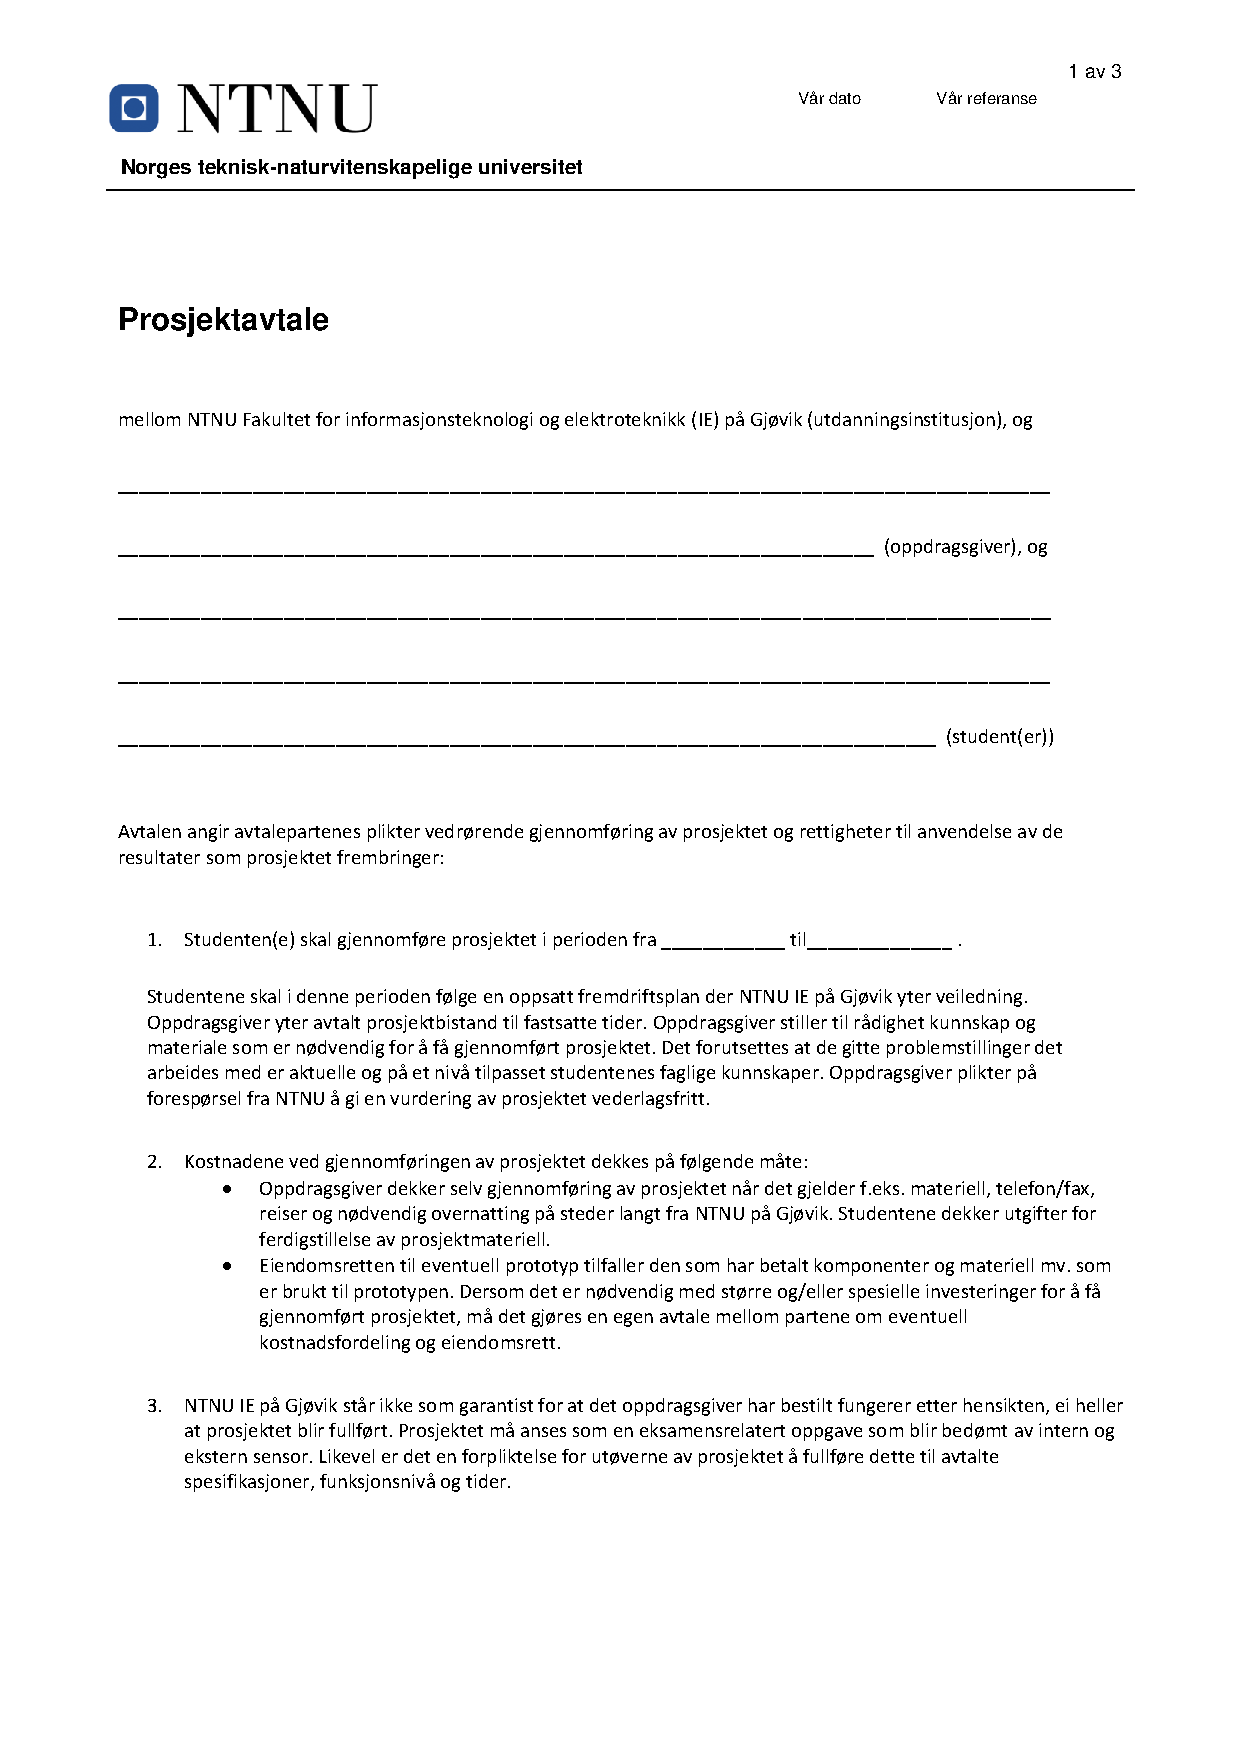
\includepdf[pages=-]{appendices/NTNUProsjektavtale.pdf}

\end{document}
